%%%%%%%%%%%%%%%%%%%%%%%%%%%%%%%%%%%%%%%%%%%%%%%%%%%%%%%%%%%%%%%%%%%%%%%%%%%%%%%%
%2345678901234567890123456789012345678901234567890123456789012345678901234567890
%        1         2         3         4         5         6         7         8
\documentclass[letterpaper, 10 pt, conference]{ieeeconf}  % Comment this line out
                                                          % if you need a4paper
%\documentclass[a4paper, 10pt, conference]{ieeeconf}      % Use this line for a4

\usepackage{float}
                                                          % paper
% uso paquete bookmark para tener bien los outlines.
\usepackage{bookmark}

% Configuro el idioma.
\usepackage[utf8]{inputenc} % Importante para mantener acentos.
\usepackage[spanish, activeacute]{babel} % Requiere: texlive-lang-spanish. Por primera vez hay que ejecutar: texconfig init> log

% Paquete para poder usar acentos en $$.
\usepackage{mathtools}
%\setmathfont{XITS math}

\usepackage{siunitx}

% package to get \url
\usepackage{hyperref}
\hypersetup{
  colorlinks=true,
  linkcolor=magenta,
  filecolor=magenta,
  citecolor=magenta,      
  urlcolor=magenta,
}

% Graficos electrónicos
\usepackage{circuitikz}

\IEEEoverridecommandlockouts                              % This command is only
                                                          % needed if you want to
                                                          % use the \thanks command
\overrideIEEEmargins
% See the \addtolength command later in the file to balance the column lengths
% on the last page of the document

\usepackage{graphicx}
\usepackage{graphics}

% styling for matlab/octave code.
\usepackage{matlab-prettifier}
% Configuracion, con esto puede agregar ñ.
\lstset{
  literate={ñ}{{\~n}}1
}

% The following packages can be found on http:\\www.ctan.org
%\usepackage{graphics} % for pdf, bitmapped graphics files
%\usepackage{epsfig} % for postscript graphics files
%\usepackage{mathptmx} % assumes new font selection scheme installed
%\usepackage{times} % assumes new font selection scheme installed
\usepackage{amsmath} % assumes amsmath package installed
%\usepackage{amssymb}  % assumes amsmath package installed

\title{\LARGE \bf Integrador TP N° 1}

\author{
  Tom\'as Vidal\\
  {\it Arquitectura de Computadoras}\\
  {\it Facultad de Ingenier\'ia, UNLP, La Plata, Argentina.}\\
  {\it 29 de Abril, 2024.}
}                                            % <-this % stops a space


% comienzo

% INTRO


% Figura
\newcommand{\image}[2] {
  \begin{figure}[H]
    \centering
    \includegraphics[width=0.43\textwidth]{./#1.png}
    \caption{#2}
    \label{fig:#1}
  \end{figure}
}

% Codigo
% \begin{lstlisting}[style=Matlab-editor]
% % el código va aca
% dispc("HELLO WORLD");
% \end{lstlisting}

\begin{document}
\maketitle
\thispagestyle{empty}
\pagestyle{empty}

%\section{INTRODUCCCI\'ON}
% TODO

\section{Bubble Sort} \label{sec:bubble_sort}
Para resolver el problema se empleó el algoritmo de \textbf{Bubble Sort}, debido a que cumple con los requerimientos, es simple, facil de implementar y, solo necesita un espacio extra de memoria. Aunque no todo es perfecto, este algoritmo implica un coste de media de $O(n^{2})$, en el mejor de los casos es $O(n)$, y en el peor nuevamente es $O(n^{2})$; esto quiere decir que si se tiene un vector con $n$ elementos, se tienen que realizar de media $n^{2}$ operaciones para ordenar este vector con este algoritmo.

\subsection{Espacio extra de memoria}
La variable \textbf{Temp}, en el código, es un espacio de memoria extra requerido (mencionado previamente en \ref{sec:bubble_sort}) que se emplea para almacenar temporalmente el dato del vector que está siendo comparado, ya que la idea del algoritmo es utilizar las mismas posiciones de memoria y no crear nuevas; por ejemplo: si se tiene el vector $[a_0, a_1, a_2]$, $a_0=1$, $a_1=-1$ y $a_2=10$ y se está ordenando $a_0$, entonces almaceno temporalmente $a_0$ y copio el valor de $a_1$ en la posición de memoria de $a_0$ (ya que quiero ordenar de menor a mayor), y luego copio el valor almacenado en la memoria temporal en la posición de memoria del dato $a_1$. Si no se hubiera empleado un espacio extra de memoria, no se hubiera podido recuperar el valor de $a_0$ para copiarlo en $a_1$.

%\subsection{Elementos de trabajo}
%Para realizar las pruebas se emplearon diversos instrumentos de laboratorio: \textit{osciloscopio}\footnote{Instrumento utilizado para visualizar y analizar formas de onda eléctricas.}, \textit{multímetro}\footnote{Dispositivo que se utiliza para medir magnitudes eléctricas como corriente, voltaje y resistencia.}, \textit{fuente regulable}\footnote{Dispositivo que proporciona una corriente o voltaje de salida regulable y estable.}, \textit{generador de funciones}\footnote{Dispositivo utilizado para generar señales eléctricas de forma controlada (en amplitud y frecuencia), como ondas sinusoidales, cuadradas, etc.}, y las placas de ensayos provistas a las cuales se las referirá como \textit{1} (ver Figura~\ref{placaDePruebas1}) y \textit{2} (ver Figura~\ref{placaDePruebas2}).
%
%\subsection{Placa de ensayos 1}
%La placa de ensayos \textbf{1} permite recrear diversas topologías de una etapa de amplificación con un amplificador operacional 741\footnote{Para ver las especificaciones vea la hoja de datos del fabricante \href{https://www.ti.com/lit/ds/symlink/lm741-mil.pdf}{https://www.ti.com/lit/ds/symlink/lm741-mil.pdf}}, esta placa es la síntesis correspondiente al diagrama circuital de la figura \ref{diagramaPlaca1}. En particular se trabajó con las topologías realimentadas negativamente\footnote{La conexión que hace la realimentación se conecta a la entrada inversora del amplificador operacional} de tal manera que una de ellas sea inversora (Fig. \ref{diagramaConfigInversora}), es decir crea un desfase de 180°; y otra no inversora (Fig. \ref{diagramaConfigNoInversora}), es decir no hay desfase. \\
%\hspace*{3pt} Las ganancias teóricas ideales de los amplificadores son $G=-\frac{R_f}{R_1}$ para la etapa inversora. Y $G=1+\frac{R_f}{R_1}$ para la no inversora.
%\begin{figure}[H]
%  \centering
%  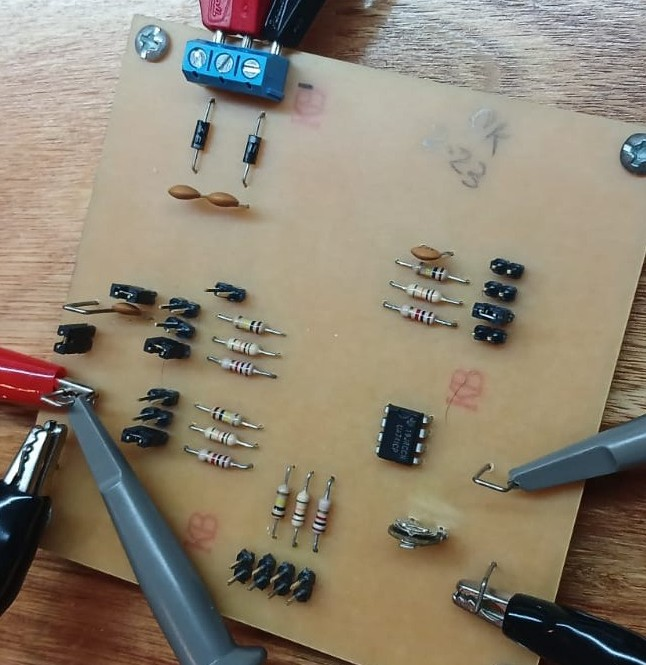
\includegraphics[width=0.43\textwidth]{./placaDePruebas1.jpeg}
%  \caption{Diagrama correspondiente a la placa de ensayos 1}
%  \label{placaDePruebas1}
%\end{figure}
%\begin{figure}[H]
%  \centering
%  % TODO
%  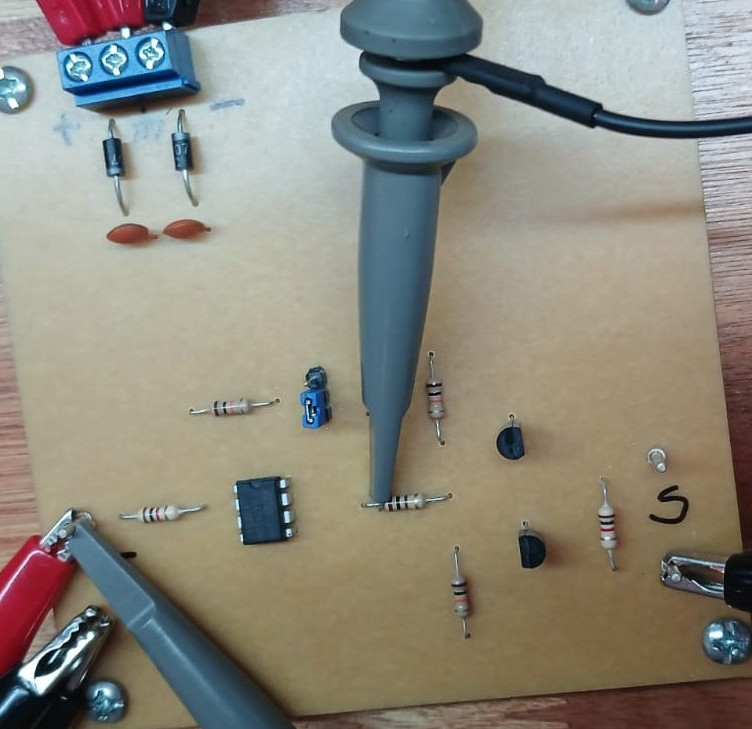
\includegraphics[width=0.43\textwidth]{./placaDePruebas2.jpeg}
%  \caption{Diagrama correspondiente a la placa de ensayos 1}
%  \label{placaDePruebas2}
%\end{figure}
%
%Para poder construir estas topologías se configuraron los \textit{jumpers}\footnote{Un \textit{jumper} o \textit{puente} es un elemento de electrónica que permite abrir o cerrar un circuito eléctrico mediante terminales.} de la placa de pruebas 1. Posteriormente se midió la entrada y la salida del circuito con las sondas del osciloscopio, canal 1 en la entrada (\textit{color amarillo en la pantalla}) y el 2 en la salida (\textit{color azul en la pantalla}). Luego se conectó a la entrada el generador de señales y se alimentó la placa (+12V, GND y -12V) con la fuente regulable. De esta manera se pudo analizar la ganancia y la frecuencia de corte de -3dB del amplificador para diferentes valores de los resistores involucrados y en las dos topologías (inversora y no inversora).
%
%\begin{figure}[H]
%   \centering
%   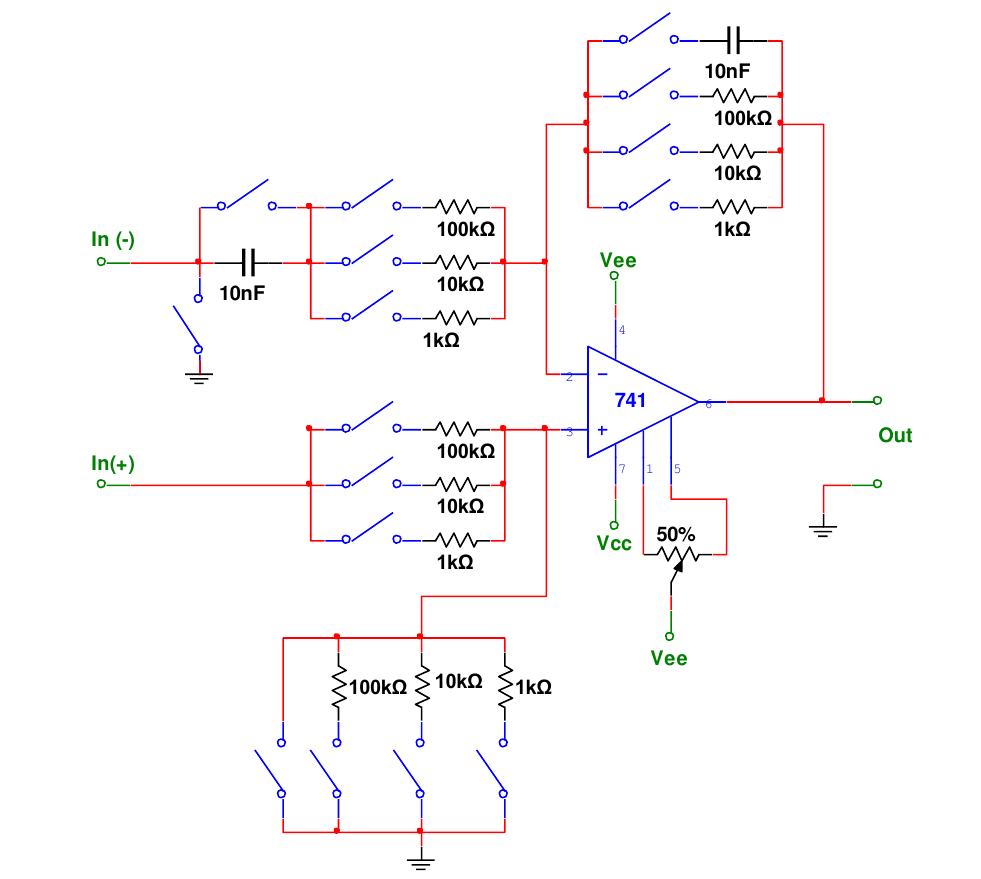
\includegraphics[width=0.43\textwidth]{./diagramaPlaca1.png}
%   \caption{Diagrama correspondiente a la placa de ensayos 1}
%   \label{diagramaPlaca1}
% \end{figure}
%
%\begin{figure}[H]
%  \centering
%  \begin{circuitikz}
%    \node[op amp] (opamp) at (0,0) {};
%    \draw (opamp.+) -- ++(-0.25,0) -- ++(0,-0.5) node[ground]{};
%    \draw (opamp.-) -- ++(-1,0) to[R=$R_1$] ++(-1.5,0) -- ++(-0.5,0) node[ocirc]{} coordinate (Vin) node[left] {$V_{in}^{+}$};
%    \draw (opamp.out) -- ++(0.25, 0) node[circ]{} -- ++(0,2) -- ++(-0.5,0) to[R=$R_f$] ++(-2,0) -- ++(-0.25,0) -- ++(0,-1.5) node[circ]{};
%    \draw (opamp.out) -- ++(1, 0) node[ocirc]{} coordinate (Vout) node[right] {$V_{out}^{+}$};
%  \end{circuitikz}
%  \caption{Amplificador operacional en configuración inversora}
%  \label{diagramaConfigInversora}
%\end{figure}
%\begin{figure}[H]
%  \centering
%  \begin{circuitikz}
%    \node[op amp] (opamp) at (0,0) {};
%    \draw (opamp.+) -- ++(-1,0) node[ocirc]{} coordinate (Vin) node[left] {$V_{in}^{+}$}; 
%    \draw (opamp.-) -- ++(-1,0) to[R=$R_1$] ++(-2,0) node[ground]{};
%    \draw (opamp.out) -- ++(0.25,0) -- ++(0,2) -- ++(-0.5,0) to[R=$R_f$] ++(-2.5,0) -- ++(0,-1.5) node[circ]{};
%    \draw (opamp.out) -- ++(0.25,0) node[circ]{} -- ++(1,0) node[ocirc]{} coordinate (Vout) node[right] {$V_{out}^{+}$};
%  \end{circuitikz}
%  \caption{Amplificador operacional en configuración no inversora}
%  \label{diagramaConfigNoInversora}
%\end{figure}
%
%\subsection{Conexiones de la placa de ensayos 1}
%Para realizar el estudio de \textit{ganancia}, \textit{desfase} y \textit{frecuencia de corte} se conectaron los sondas del osciloscopio a la entrada (canal 1, amarillo), y a la salida (canal 2, azul). De esta manera se puede calcular por comparación de la señal de entrada y salida los parámetros deseados. En todos los casos la señal de entrada fue una sinusoide de amplitud de 100mV y frecuencia de 1kHz. Para calcular la frecuencia de corte, el método empleado fue incrementar la frecuencia gradualmente hasta alcanzar un 70\% de la tensión inicial de salida, ya que esa es la proporción que cae aproximadamente en -3dB (el valor exacto sería $10^{-3/20} \approx 0.7079$).
%
%\subsection{Resultados placa de ensayos 1}
%\begin{table}[H]
%\centering
%\caption{Resultados de la topología inversora}
%\label{tab:resultadosInversora}
%\begin{tabular}{|c|c|c|c|c|}
%\hline
%$R_{1} (\unit{\kilo\ohm})$ & $R_{f} (\unit{\kilo\ohm})$ & $G$ (V/V) & $f_{-3dB}$ (\unit{\kilo\hertz}) & $|G.f_{-3dB}|$ \\
%\hline
%1 & 1 & -1 & 800 & 800 \\
%1 & 10 & -10 & 78 & 780 \\
%1 & 100 & -100 & 8 & 800 \\
%\hline
%\end{tabular}
%\end{table}
%\begin{table}[H]
%\centering
%\caption{Resultados de la topología no inversora}
%\label{tab:resultadosNoInversora}
%\begin{tabular}{|c|c|c|c|c|}
%\hline
%$R_{1} (\unit{\kilo\ohm})$ & $R_{f} (\unit{\kilo\ohm})$ & $G$ (V/V) & $f_{-3dB}$ (\unit{\kilo\hertz}) & $|G.f_{-3dB}|$ \\
%\hline
%1 & 1 & 2 & 381 & 762 \\
%1 & 10 & 11 & 75 & 825 \\
%1 & 100 & 101 & 8 & 808 \\
%\hline
%\end{tabular}
%\end{table}
%
%De los resultados en las tablas \ref{tab:resultadosInversora} y \ref{tab:resultadosNoInversora} se puede observar que el producto \textbf{ganancia - ancho de banda} se conserva, a pesar de que hay una \textit{``gran''} dispersión en los resultados debido a la forma en que se hicieron las mediciones, pero se puede establecer una media de los datos como $\overline{|G \cdot f_{\text{-3dB}}|} = 795.83 \approx 800 $.
%
%\section{Análisis de No Linealidad}
%Con la placa de ensayos 2, cuya disposición de elementos se puede observar mejor en su diagrama circuital \ref{diagramaPlaca2}, se analizó con el osciloscopio la no linealidad que se presenta entre la entrada y la salida de la placa de ensayos 2 cuando no se realimenta desde la salida, es decir el \textit{jumper} se encuentra entre los terminales 2 y 3, el resultado se puede apreciar en la imagen \ref{imagen:nolinealidad}
%
%\begin{figure}[H]
%   \centering
%   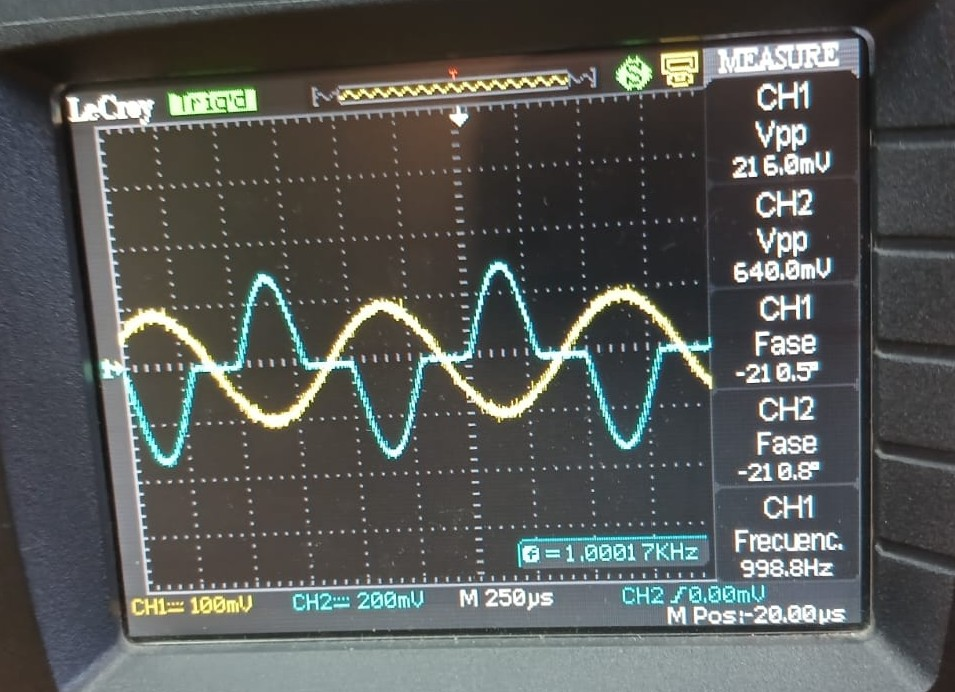
\includegraphics[width=0.43\textwidth]{./nolinealidad2.jpeg}
%   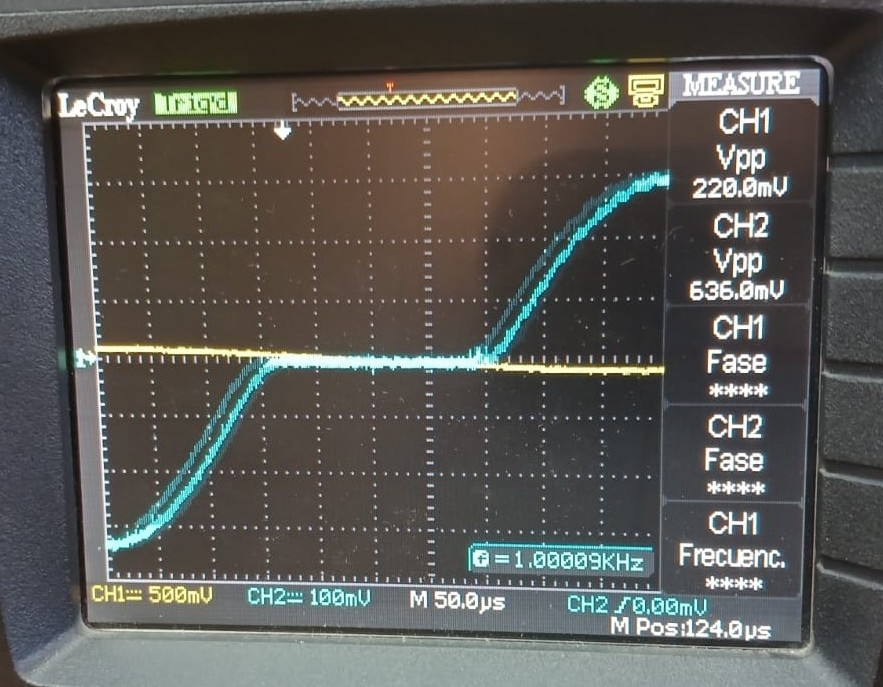
\includegraphics[width=0.43\textwidth]{./nolinealidad.jpeg}
%   \caption{Se observa la no linealidad en la señal de salida (azul)}
%   \label{imagen:nolinealidad}
% \end{figure}
%
%\begin{figure}[H]
%   \centering
%   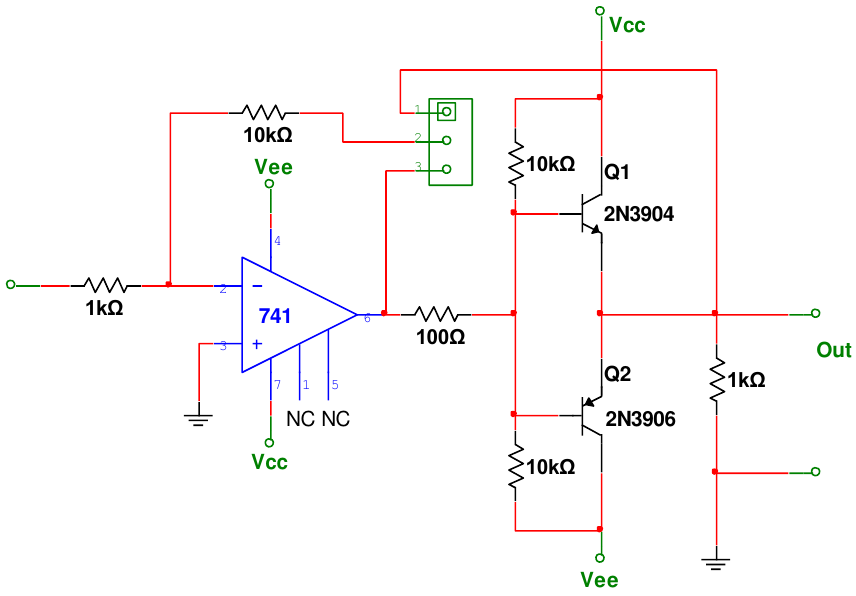
\includegraphics[width=0.43\textwidth]{./diagramaPlaca2.png}
%   \caption{Diagrama correspondiente a la placa de ensayos 2}
%   \label{diagramaPlaca2}
% \end{figure}
%
% El punto de no linealidad refiere a la parte donde es más horizontal la señal de salida, ya que no hay amplificación lineal en la salida para una señal de entrada, esto es debido a cómo se polarizan los transistores NPN y PNP. Pero luego de realimentar negativamente la salida (es decir, una parte de la señal de salida ingresa a la entrada no inversora del amplificador operacional), haciendo una conexión con el \textit{jumper} entre los terminales 1 y 2, se puede observar que la no linealidad se hace \textit{``insignificante''}, y por lo tanto el sistema es más estable; los resultados se pueden apreciar en la imagen \ref{imagen:linealidad}.
%
%\begin{figure}[H]
%   \centering
%   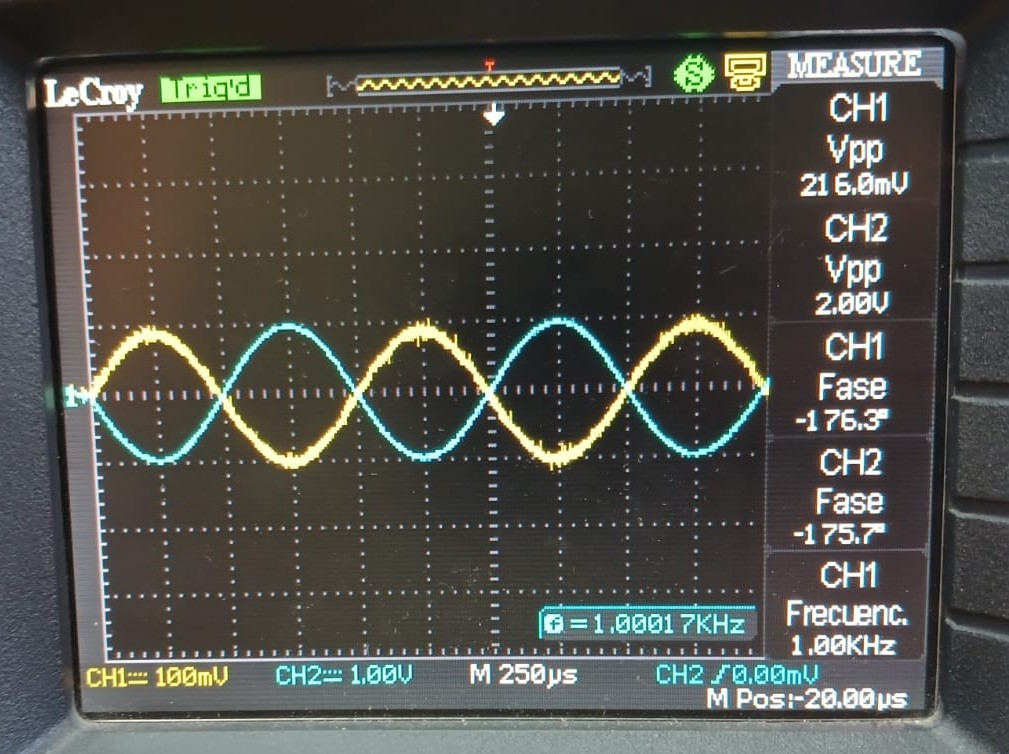
\includegraphics[width=0.43\textwidth]{./linealidad2.jpeg}
%   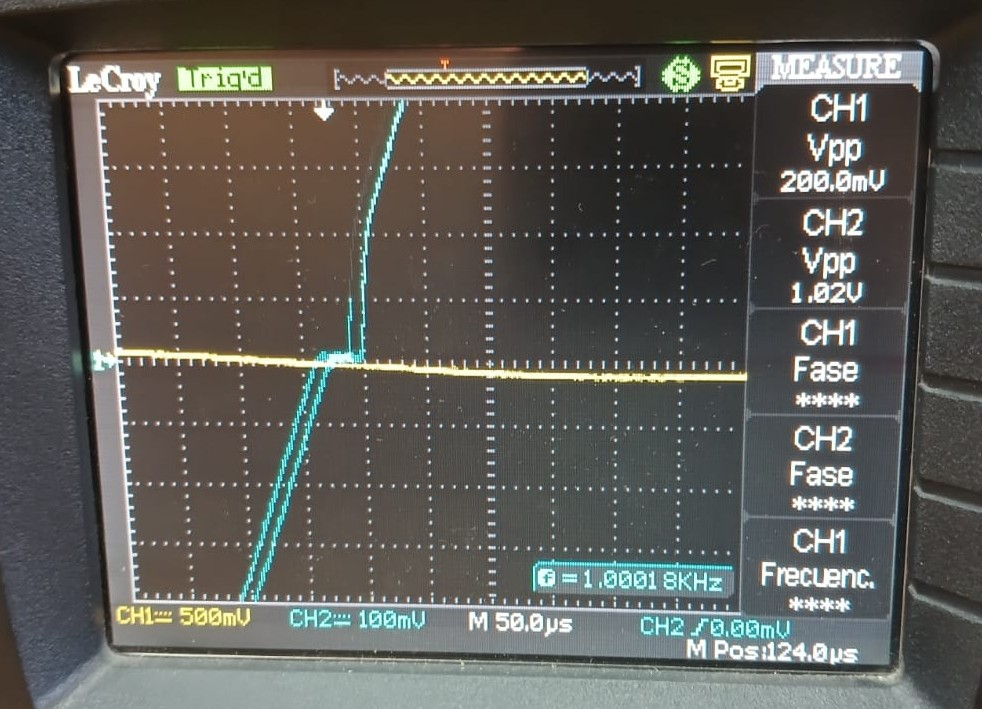
\includegraphics[width=0.43\textwidth]{./linealidad.jpeg}
%   \caption{Se observa la mejora de linealidad en la señal de salida (azul)}
%   \label{imagen:linealidad}
% \end{figure}

% \begin{thebibliography}{99}

% TODO
% \bibitem{tftd_tp5}TODO
% \bibitem{tftd_tp5}ANÁLISIS DE SISTEMAS Y SE\~{n}ALES - A\~{n}O 2022, Práctica 5 Transformada de Fourier de Tiempo Discreto (TFTD), Serie Discreta Fourier (SDF).
% \bibitem{tftd_teoria}ANÁLISIS DE SISTEMAS Y SE\~{n}ALES - A\~{n}O 2022, Filminas de teor\'ia 5: Transformada de Fourier de Tiempo Discreto (TFTD).
%
% \end{thebibliography}

\end{document}
